% ------------------------------------------------------------------------
% Senac Tex: Modelo de Trabalho Academico para o Centro Universitário
% Senac
% ------------------------------------------------------------------------

% ========================================================================
% CONFIGURAÇÃO DO DOCUMENTO
% ========================================================================


\documentclass[
	% -- opções da classe memoir --
	12pt,				% tamanho da fonte
	openright,			% capítulos começam em pág ímpar (insere página vazia caso preciso)
	oneside,			% para impressão em verso e anverso. Oposto a oneside
	a4paper,			% tamanho do papel. 
	% -- opções da classe abntex2 --
	%chapter=TITLE,		% títulos de capítulos convertidos em letras maiúsculas
	%section=TITLE,		% títulos de seções convertidos em letras maiúsculas
	%subsection=TITLE,	% títulos de subseções convertidos em letras maiúsculas
	%subsubsection=TITLE,% títulos de subsubseções convertidos em letras maiúsculas
	% -- opções do pacote babel --
	english,			% idioma adicional para hifenização
	brazil				% o último idioma é o principal do documento
	]{abntex2}

% ---
% Pacotes básicos 
% ---
\usepackage{tikz}
\usepackage{lmodern}			% Usa a fonte Latin Modern			
\usepackage[T1]{fontenc}		% Selecao de codigos de fonte.
\usepackage[utf8]{inputenc}		% Codificacao do documento (conversão automática dos acentos)
\usepackage{lastpage}			% Usado pela Ficha catalográfica
\usepackage{indentfirst}		% Indenta o primeiro parágrafo de cada seção.
\usepackage{color}				% Controle das cores
\usepackage{graphicx}			% Inclusão de gráficos
\usepackage{microtype} 			% para melhorias de justificação
\usepackage{listings}
\usepackage{amsmath} % Required for the split environment
\usepackage{indentfirst}
\usepackage[top=3cm, bottom=2cm, left=3cm, right=2cm]{geometry}

% ---
% Pacotes de citações
% ---
\usepackage[brazilian,hyperpageref]{backref}	 % Paginas com as citações na bibl
\usepackage[alf]{abntex2cite}	% Citações padrão ABNT

% CONFIGURAÇÕES DE PACOTES

% Configurações do pacote backref
% Usado sem a opção hyperpageref de backref
\renewcommand{\backrefpagesname}{Citado na(s) página(s):~}
% Texto padrão antes do número das páginas
\renewcommand{\backref}{}
% Define os textos da citação
\renewcommand*{\backrefalt}[4]{
	\ifcase #1 %
		Nenhuma citação no texto.%
	\or
		Citado na página #2.%
	\else
		Citado #1 vezes nas páginas #2.%
	\fi}%

\usetikzlibrary{arrows.meta, shapes.geometric}

% Define custom colors for TikZ diagrams
\definecolor{w}{rgb}{1,1,1}    % white
\definecolor{b}{rgb}{0,0,0}    % black
\definecolor{g}{rgb}{0.7,0.7,0.7}  % gray

% Informações de dados para CAPA e FOLHA DE ROSTO
\titulo{Titulo do Trabalho}
\autor{Lucas da Mata Guimarães}
\local{São Paulo - Brasil}
\data{2025}
\orientador{Nome do Orientador}
%\coorientador{Nome do Coorientador}
\instituicao{
  Centro Universitário Senac - Santo Amaro
  \par
  Bacharelado em Ciência da Computação
}
\tipotrabalho{Trabalho de Conclusão de Curso}
% O preambulo deve conter o tipo do trabalho, o objetivo, 
% o nome da instituição e a área de concentração 
\preambulo{Monografia apresentada na disciplina Trabalho de Conclusão de Curso, como parte dos requisitos para obtenção do título de Bacharel em Ciência da Computação.}

% Configurações de aparência do PDF final

% alterando o aspecto da cor azul
\definecolor{blue}{RGB}{41,5,195}

% formato de código
\lstdefinestyle{psceudo}{
    language=C,
    basicstyle=\ttfamily\small,
    keywordstyle=\bfseries, 
    numbers=left, 
    numberstyle=\tiny, 
    stepnumber=1,
    captionpos=t,
    tabsize=2,
    breaklines=true,
    showstringspaces=false
}

% informações do PDF
\makeatletter
\hypersetup{
     	%pagebackref=true,
		pdftitle={\@title}, 
		pdfauthor={\@author},
    	pdfsubject={\imprimirpreambulo},
	    pdfcreator={LaTeX with abnTeX2},
		pdfkeywords={abnt}{latex}{abntex}{abntex2}{trabalho acadêmico}, 
		colorlinks=true,       		% false: boxed links; true: colored links
    	linkcolor=blue,          	% color of internal links
    	citecolor=blue,        		% color of links to bibliography
    	filecolor=magenta,      		% color of file links
		urlcolor=blue,
		bookmarksdepth=4
}
\makeatother

% Espaçamentos entre linhas e parágrafos 

% O tamanho do parágrafo é dado por:
\setlength{\parindent}{1.25cm}

% Controle do espaçamento entre um parágrafo e outro:
\setlength{\parskip}{0.2cm}

\SingleSpacing
\makeatletter
\let\@fnsymbol\@arabic
\makeatother

% compila o indice
\makeindex

\begin{document}

% Retira espaço extra obsoleto entre as frases.
\frenchspacing

% ========================================================================
% CAPA
% ========================================================================
\imprimircapa

% ========================================================================
% FOLHA DE ROSTO
% ========================================================================
\imprimirfolhaderosto

% ========================================================================
% DEDICATÓRIA
% ========================================================================
 \begin{dedicatoria}
   \vspace*{\fill}
   \centering
   \noindent
   \textit{ Texto da dedicatória.} \vspace*{\fill}
 \end{dedicatoria}

% ========================================================================
% AGRADECIMENTOS
% ========================================================================
 \begin{agradecimentos}
 Texto de agradecimento.

 \end{agradecimentos}

% ========================================================================
% EPÍGRAFE
% ========================================================================
 \begin{epigrafe}
     \vspace*{\fill}
 	\begin{flushright}
 		\textit{``A vingança nunca é plena, \\
 		mata a alma e a envenena. \\
 		(MADRUGA, Seu, Chaves)}
 	\end{flushright}
 \end{epigrafe}

% ========================================================================
% RESUMO
% ========================================================================
\setlength{\absparsep}{18pt} % ajusta o espaçamento dos parágrafos do resumo
\begin{resumo}

Texto do resumo

\textbf{Palavras-chaves}: palavra-chave 1, palavra-chave 2, palavra-chave 3.
\end{resumo}

% ========================================================================
% ABSTRACT
% ========================================================================
\begin{resumo}[Abstract]
 \begin{otherlanguage*}{english}
    Abstract text in english
   
   \textbf{Key-words}: keyword 1, keyword 2, keyword 3
 \end{otherlanguage*}
\end{resumo}

% ========================================================================
% LISTA DE ILISTRAÇÕES
% ========================================================================
\pdfbookmark[0]{\listfigurename}{lof}
\listoffigures*
\cleardoublepage

% ========================================================================
% LISTA DE TABELAS
% ========================================================================
\pdfbookmark[0]{\listtablename}{lot}
\listoftables*
\cleardoublepage

% ========================================================================
% LISTA DE ABREVIATURAS E SIGLAS
% ========================================================================
\begin{siglas}
  \item[GAM] Generalized Additive Models
  \item[GLM] Generalized Linear Model
  \item[MARS] Multivariate Adaptive Regression Spline
  \item[ML] Maximum likelihood
\end{siglas}

% ========================================================================
% SUMÁRIO
% ========================================================================
\pdfbookmark[0]{\contentsname}{toc}
\tableofcontents*
\cleardoublepage

\textual
% ========================================================================
% INTRODUÇÃO
% ========================================================================
\chapter{Introdução}

\section{Contexto}

O uso de modelos computacionais, na Biologia, possibilita o avanço de diferentes
estudos \cite{modelagem_comp}. Uma destas aplicações são os modelos de distribuição 
de especies, que são capazes de fornecer uma visualização da situação 
da fauna e flora de determinada região, podendo mostrar como estas estão se 
comportando no decorrer do tempo \cite{speciesDistributionModels}.

Entre esses modelos, os mais utilizados são o Generalized Additive Models (GAM) \cite{GAM}
e o Generalized Linear Model (GLM) \cite{GLM}. Esses dois modelos usam uma função para 
estabelecer uma relação entre a média da variável de resposta e uma função 'suavizada'
das variáveis explanatórias, sendo o GLM uma extenção de modelos lineares que não
forçam o dado a escalas não naturais, e o GAM uma extenção semi-parametrizada do GLM,
tendo a capacidade de atuar com relações não lineares e não monótonas \cite{GAMeGLM_especie_estudo}. 

Já o Multivariate Adaptive Regression Spline (MARS) combina partição recursiva e ajustes
por splines, de modo a manter seus aspectos positivos, enquanto sendo menos vulneravel a 
suas propriedades não favoraveis. Gerando um conjunto de regras para prever
valores futuros apartir de uma análise regressiva. \cite{MARS} 

Sendo as aplicações destes modelos encontradas códificadas na linguagem de programação R, que por
sua vez é a linguagem de programação mais utilizada quando tratamos de ciência de dados, sendo conhecida
como a lingaugem mais robusta para a área de dados, tendo sido pensada para o uso em cálculos e
análises estatísticas \cite{linguagem_r}.

Porém, estes modelos podem requisitar uma alta demanda de processamento e memória do computador hospedeiro, 
como citado por \cite{modelagem_comp}, ponto este, que não é repassado nos trabalhos referentes a análise 
ou uso dos modelos citados. Logo, mesmo com a facilidade de se adquirir um computador, tais modelos
requerem computadores de alto desempenho para serem treinados, tornando esse processo lento ou criando 
a necessidade de se alugar maquinas virtuais para está finalidade \cite{global_cloud_maketing}. 

E quando se coloca a necessidade de se manter um controle das populações de espécies, dentro ou próximo
a centros urbanos, a velocidade de preparo destes modelos se torna mais critica, já que é necessário ir
desde a coleta dos dados, ao treino e validação do modelo, e análise dos resultados obtidos.
 
\section{Justificativa}

Identificar a distribuição de espécies em um dado ambiente, em um determinado intervalo de tempo, 
é importante para termos noção de como as espécies estão respondendo a mudanças no ambiente, no aumento 
ou diminuição de outra espécie.

Uma vez que essas mudanças podem ser geradas pela ação humana, na construção civil e de infraestrutura 
\cite{impactConstruction}, conseguir estimar o impacto dessas ações é vantajoso para a preservação de espécies.

Além disso, estas abordagens aumentam as possibilidades para integrar a infraestrutura necessária, 
contribuindo para a sobrevivência de espécies que estão em níveis populacionais baixos.

Modelos estatísticos, que tem a capacidade de demonstrar estes eventos, aplicam de maneiras diferentes algumas 
linhas de abordagem. O Generalized Additive Models (GAM), Generalized Linear Model (GLM), e o 
Multivariate Adaptive Regression Spline (MARS), ambos com uma abordagem de Maximum likelihood (ML), 
variando em sua capacidade de atuar com um determinado tipo de dado e o custo levado para seu treinamento 
e utilização \cite{predPerform33models}.

Modelos que são utilizados na modelagem de distribuição de espécies necessitam de uma quantidade elevada de dados 
\cite{sampleSize}, de ocorrência e ausência, sendo os dados de ausência não necessários em todos os tipos de modelos.

Nem todas as espécies são facilmente modeláveis devido à dificuldade de coleta de dados, seja pela sua raridade ou habitat 
\cite{especiesDificies}. A colaboração de cidadãos na coleta de dados pode auxiliar na identificação de áreas prioritárias 
para pesquisa. Portanto, a identificação de bons modelos que trabalham com esses dados é vantajosa.

Dentro destes modelos, além da quantidade e tipo de dados necessários, precisamos levar em consideração, o custo necessário de 
processamento e o espaço de memória utilizado pelo mesmo, para este fim utilizamos a análise de complexidade 
e espaço \cite{introductionAlgorthms}, já que um modelo mais barato nesse quesito pode ser criado em computadores 
mais acessíveis \cite{introductionAnalysis}, e ser possível a construção de mais de um modelo de modo simultâneo.

Os pontos levantados anteriormente podem afetar a acurácia de um modelo, mesmo atendendo os requisitos, 
de pouco adianta se o mesmo nos entrega respostas que induzem ao erro. Identificar um modelo que tenham uma boa acurácia, 
quando trabalham somente com dados de ocorrência, assim como uma melhor avaliação computacional, se vê vantajoso para 
situações em que queremos criar uma análise inicial de um determinado senário.

\section{Objetivo}

Este trabalho tem como objetivo avaliar e comparar a implementação encontrada nas bibliotecas mda e mgcv da linguagem R, dos modelos
de distribuição de espécies, GAM, GML e MARS, levantando o custo computacional de cada um destes apartir de uma análise de 
complexidade e espaço. Encontrando um modelo que melhor aprensente um equilibrio entre a acurácia e o custo computacional.

\subsection{Objetivos Específicos}

\begin{enumerate}
	\item Análise de complexidade e espaço dos modelos.
	\begin{itemize}
		\item Generalized Addtive Model;
		\item Generalized Linear Model;
		\item Multivariate Adaptive Regression Spline;
	\end{itemize}
	\item Avaliação da acurácia dos modelos com dados de ocorrência.
	\item Comparação dos modelos.
	\item Avaliação dos modelos com base na relação custo x acurácia.
\end{enumerate}

% ========================================================================
% REVISÃO BIBLIOGRÁFICA
% [ ] Aprofundar nos modelos
% [ ] Metodos de avaliação de modelo
% [x] Cormam para a analise de complexidade
% [ ] Análise de espaço
% [x] Fonte da tabela
% [ ] Primeira pessoa
% ========================================================================


\chapter{Revisão Bibliográfica}

\section{Modelos Computacionais}

Modelos computacionais são modelos que representam fenômenos de modo simplificado, gerando uma aproximação
do evento real, tendo em vista a visualização ou entendimento de determinado fenômeno, codificados em 
alguma linguagem computacional para ser executado em um computador. Estes modelos podem ser criados
por especialistas utilizando de equações matemáticas ou, automaticamente utilizando de técnicas de
inteligência artificial. \cite{modelos_computacionais}

Ao processo de criação destes modelos, damos o nome de modelagem computacional, podendo ser aplicado em
qualquer situação onde uma análise de um sistema complexo se vê necessária, sendo suas principais
aplicações encontradas nas seguintes áreas, como apresentado por \cite{modelagem_computacional}:

\begin{enumerate}
	\item \textbf{Ciência e Pesquisa}: Permite o teste de hipóteses de maneira mais rápida e eficiente.
	\item \textbf{Engenharia}: Essencial para projetos de larga escala, utilizada para testar estruturas antes de
	começar sua construção.
	\item \textbf{Medicina}: Permite a modelagem de epidemias, assim prevendo como doenças podem se espalhar em dada
	população, ajudando a planejar métodos de controle.
\end{enumerate}

O tipo da modelagem depende do tipo de fenômeno ou problema que queromos tratar, onde os tipos principais
segundo \cite{modelagem_computacional} são:

\begin{enumerate}
	\item \textbf{Modelagem determinística}: O comportamento do sistema é previsível, onde os mesmos parâmetros de 
	entrada sempre produzem os mesmos resultados. Mais visto no campo da Física e Engenharia, onde os 
	fenômenos naturais seguem um conjunto de regras bem definido.
	\item \textbf{Modelagem estocástica}: Inclui elementos de incerteza e aleatoriredade, o sistema pode apresentar
	resultados diferentes para o mesmo conjunto de parâmetros de entrada. Comumente usada onde o acaso 
	desempenha um papel importante, como na Biologia e Economia.
	\item \textbf{Modelagem dinâmica}: Focada em sistemas que mudam ao longo do tempo, essencial em áreas como a
	Ecologia e Epidemiologia, onde se é preciso prever a evolução de sistemas biológicos ou a propagação
	de doenças. 
\end{enumerate}

% Transição abrupita, possivel melhora?

\subsection{Modelos Lineares}

Modelos lineares são modelos que preveem uma respota linear utilizando de base a relação entre o resultado
e as propriedades dadas como parâmetros. Sendo uma opção mais simples, possuem propriedades mais fáceis de
serem entendidas e um tempo de desenvolvimento mais curto quando comparado a outros tipos de modelos,
como redes neurais, ou árvores de decisão, empregadas no mesmo problema. \cite{modelos_lineares}

A linearidade destes modelos, implica que matematicamente a variação dos parâmetros independentes não
possuem relações entre si, e podem ser separados em dois grupos clássicos \cite{tipos_modelos_lineares}.
\begin{itemize}
	\item \textbf{Modelos de Regressão}:
	Este grupo é utilizado para modelar relações entre variáveis quantitativas, que são um conjunto de
	valores de possível representação numérica, indicando quantidade ou magnitude. Com o intuito de estimar
	parâmetros, explicando relação ou para fazer predições.
	\item \textbf{Modelos de Análise de Váriancia}:
	Estes modelos tem como questão principal comparar a importância de fatores sobre o comportamento da
	variável de resposta. Para encontrar a relação entre grupos de análise, de modo a indentificar oque
	gera a diferença entre os grupos estudados.
\end{itemize}

Ambas as abordagens ao modelo linear, irão gerar uma regressão linear, que é um modelo matemático que 
descrevem a relação entre as váriveis dependentes e independentes usadas, tendo a possibilidade de ser
representado graficamente. Podendo ser de dois tipos, simples ou múltipla.

Na regressõa linear simples, queremos estimar os valor de $a$ e $b$ da equação da reta, $y$ = $a$ + $bx$, 
apartir de um conjunto de dados $x$ e $y$, onde $y$ representa a váriavel dependete e $x$ á váriavel 
independente, que melhor represente a relação entre $x$ e $y$. Em outras palavras, queremos estimar a 
inclinação da reta, esta que nos indica o efeito em $y$ das mudanças ocorridas em $x$ 
\cite{modelos_regressao_linear}.

A essa reta, é dado o nome de reta de regressão linear, está que depende de cinco estátisticas básicas
\cite{modelos_regressao_linear}:

\begin{enumerate}
	\item Média de $X$: $\overline{X} = \frac{1}{N} \sum_{i=1}^{N} X_i$;
	\item Desvio padrão de $X$: $S_x = \sqrt{ \frac{1}{N} \sum_{i=1}^{N} (X_i - \overline{X})^2 }$;
	\item Média de $Y$: $\overline{Y} = \frac{1}{N} \sum_{i=1}^{N} Y_i$;
	\item Desvio padrão de $Y$: $S_y = \sqrt{ \frac{1}{N} \sum_{i=1}^{N} (Y_i - \overline{Y})^2 }$;
	\item Correlação de $X$ e $Y$: $r = \frac{1}{n} \sum_{i=1}^{N} \frac{X_i - \overline{X}}{S_X} . \frac{Y_i - \overline{Y}}{S_Y}$
\end{enumerate}

Com estas estátisticas podemos traçar a reta de regressão, sabendo que esta passa pelo ponto médio
($\overline{X}, \overline{Y}$). A inclinação da reta será dada por:

\begin{equation}
	\label{inclinacao_reta}
	\beta_1 = \frac{r.S_y}{S_x}
\end{equation}

E o intercepto da reta de regressão, onde a reta corta um dos eixos do plano cartesiano, 
será dado por:

\begin{equation}
	\label{intercepto_reta}
	\beta_0 = \overline{Y} - \beta_1 \overline{X}
\end{equation}

Assim resultamos na seguinte equação:

\begin{equation}
\label{eq_reg_simples}
	Y = \beta_0 + \beta_1X
\end{equation}

Onde:
\begin{itemize}
	\item ($X$) é a variável independente;
	\item ($Y$) é a variável dependente;
	\item ($\beta_0$) é o intercepto da reta;
	\item ($\beta_1$) é a inclinação da reta. 
\end{itemize}

Porém, a equação \ref{eq_reg_simples} ainda não proporciona os valores de $Y$, mesmo possuindo
os valores para $\beta_0$ e $\beta_1$, visto que não é apenas a váriavel $X$ que afeta os valores de
$Y$ quando tratamos de ocorrência no mundo real, assim incluimos um termo de erro $\epsilon$, que é
o erro que se comete ao estimar os valores de $Y$ por meio da variável $X$ \cite{modelos_regressao_linear}.

\begin{equation}
	\label{eq_reg_simples_erro}
	Y = \beta_0 + \beta_1X + \epsilon
\end{equation}

Agora com a equação \ref{eq_reg_simples_erro}, podemos criar a reta de regressão, que pode ser
representada graficamente, possuindo uma estrutura semelhante ao gráfico a seguir:

\begin{figure}[htb]
    \centering
    \caption{\label{Regressão Linear Simples}Regressão Linear Simples}
    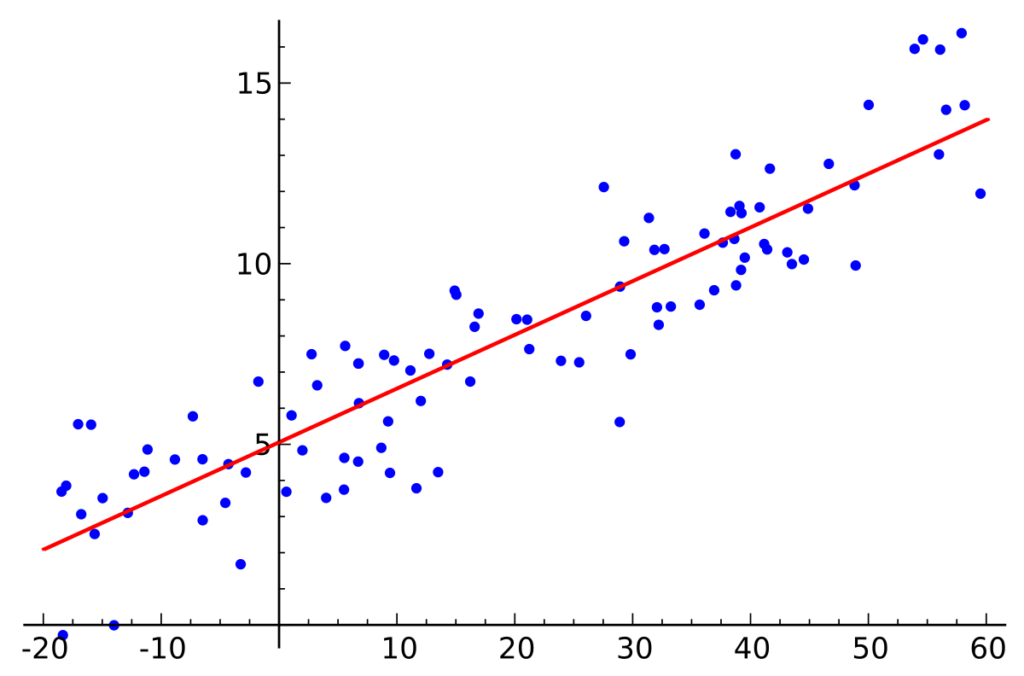
\includegraphics[width=0.50\textwidth]{../Imgs/reg_linear_simples.png}
    \legend{Fonte: \citeonline{regressao_linear}}
\end{figure}

A equação \ref{eq_reg_simples_erro}, pode ser escrita de forma mais geral. Visto que em nosso dados
podemos trabalhar com conjuntos de valores, agrupando valores de $Y$ distintos, para cada valor de $X$.
Por exemplo, dados que representam a qualidade de vida nos estados brasileiro com o número de postos 
de saúde. Assim a equação \ref{eq_reg_simples_erro} ficaria \cite{modelos_regressao_linear}:

\begin{equation}
	\label{eq_reg_simples_geral}
	Y_i = \beta_0 + _beta_iX_i + \epsilon_i
\end{equation}

Onde:
\begin{itemize}
	\item ($i$) representa um agrupamento de dados, um estado brasileiro seguindo o exemplo dado acima;
	\item ($Y_i$) é a variável dependente;
	\item ($X_i$) é a variável independente, representaria o número de postos de saúde em dado estado.
	\item ($\beta_0$) é o intercepto;
	\item ($\beta_1$) é a inclinação, e o efeito médio de $X_i$ sobre $Y_i$;
	\item ($\epsilon$) é o erro médio ao se estimar $Y_i$ por meio de $X_i$;
\end{itemize}

Já quando tratamos da regressão linear múltipla, é levado em conta que outros fatores podem afetar a
váriavel de resposta, este que também podem ser correlacionados com a váriavel independente. A formula
para este modelo de regressão, pode ser representa da seguinte forma, onde temos $k$ variáveis, 
explicativas \cite{modelos_regressao_linear}:

\begin{equation}
	\label{rq_reg_multipla}
	Y = \beta_0 + \beta_1X_1 + \beta_2X_2 + ... + \beta_kX_k + \epsilon
\end{equation}

Onde:
\begin{itemize}
	\item ($\beta_0$) é o intercepto;
	\item ($\beta_1,...,\beta_k$) são "inclinações", mesmo que na prática não sejam inclinações da função
	\item ($\epsilon$) é o termo de erro.
\end{itemize}

Aqui temos $\beta_1$ até $\beta_k$ como coeficientes parcias da regressão \cite{modelos_regressao_linear}. Neste caso, a visualização por
meio de um gráfico, fica comprometida, visto que temos um número $k$ de $X$, para ilustrar, usemos uma
situação onde temos dois $X$, aqui podemos representar os valores por um gráfico de três dimenções.

\begin{figure}[htb]
    \centering
    \caption{\label{Regressão Linear Multipla}Regressão Linear Multipla}
    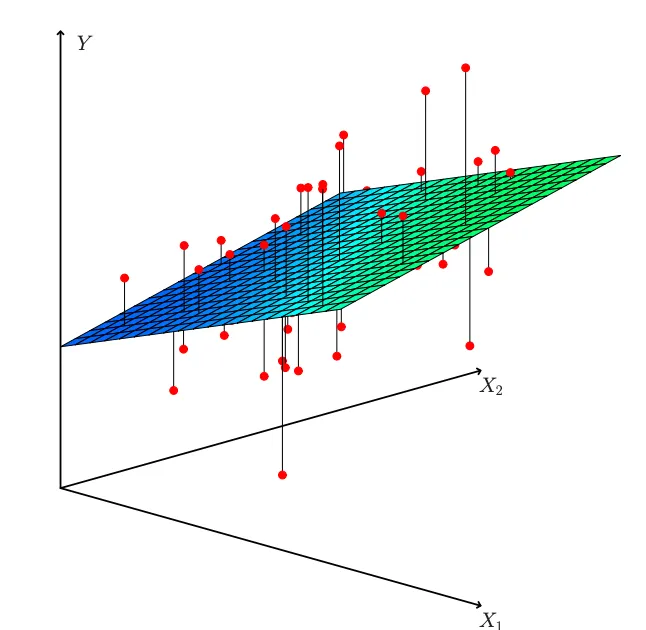
\includegraphics[width=0.50\textwidth]{../Imgs/reg_linear_multipla.png}
    \legend{Fonte: \citeonline{regressao_linear_multipla_img}}
\end{figure}

Quando temos mais de dois valores de $X$ a representação gráfica fica confusa para o entendimento humano,
mas ainda podemos tratar o problema como uma reta.

\subsection{Acurácia}

A acurácia é um modo de avaliar a performance de um modelo, assim identificando se seus resultados podem
ser considerados válidos ou não. Para chegarmos na acurácia utilizamos da seguinte formula \cite{acuracia}:

\begin{equation}
	\label{acuracia}
	A = \frac{PC}{TP}
\end{equation}

Onde:
\begin{itemize}
	\item ($A$) é a Acurácia
	\item ($PC$) é o total de Previsões Corretas, encontrada pela soma, ($Positivos Verdadeiros + Negativos Verdadeiros$);
	\item ($TP$) é o Total de Previsões, encontrada pela soma, ($PC + Falsos Verdadeiros + Falsos Negativos$).
\end{itemize}

Como a acurácia incorpora por completo a matriz de confusão \ref{Matriz de Confusão}, em um conjunto de dados equilibrado, 
com uma quantidade de exempols semelhante para as duas classes, ela pode ser usada como uma médida grosseira da qualidade 
de um modelo \cite{acuracia_matriz}.

Onde temos mais exemplos de uma classe doque de outras, é importante considerar outras métricas de avaliação, já que esses
modelos são considerados desbalanceados \cite{acuracia}.

Uma matriz de confusão, por usa vez, é uma representação binária em forma de matriz dos resultados possíveis ao se utilizar 
o modelo, sendo representada da seguinte forma:

\begin{table}[h!]
	\centering
	\caption{\label{Matriz de Confusão}Matriz de Confusão}
	\begin{tabular}{|c|c|c|}
	\hline
					  & Verdadeiro Positivo & Verdadeiro Negativo   \\ \hline
	Positivo Previsto & Positivo Verdadeiro & Falsos Positivos      \\ \hline
	Negativo Previsto & Falsos Negativos    & Negativos Verdadeiros \\ \hline
	\end{tabular}
	\legend{Fonte: \cite{acuracia}}
\end{table}

Onde:
\begin{itemize}
	\item \textbf{Positivos Verdadeiros}: São as classificações positivas corretas;
	\item \textbf{Falsos Positivos}: São positivos que foram erroneamente classificados como negativos;
	\item \textbf{Falsos Negativos}: São negativos que foram erroneamente classificados como positivos;
	\item \textbf{Negativos Verdadeiros}: São as classificações negativas corretas;
\end{itemize}

\subsection{Modelos de Distribuição de Especies}

Definimos um Modelos de Distribuição de Especies, SDM (Spice Distribution Model), como um modelo que relaciona dados de 
distribuição de especies, com informações sobre as caraceristicas ambientais e/ou epaciais de certas localidades, podendo 
ser usados para entender e/ou prever a distribuição de uma espécie em uma dada locaclidade \cite{speciesDistributionModels}.

SDMs comtemporaneos combinan conceitos de ecologia e historia natural com os avanços mais recentes em estatísticas e
tecnologia da informação, as raizes destes modelos são encontradas nos estudos mais antigos que descrevem padrões
biológicos em termos de relações com geografia e/ou gradientes ambientais, e estudos que indicam a resposta individual
de especies para seus ambientais, proveem um forte argumento conceitual para se modelar especies de modo individual 
\cite{speciesDistributionModels}.

Segundo \cite{tiposDados_sdm} as principais fontes de inforamções para a criação destes modelos são: 
\begin{itemize}
	\item Dado de ocorrência: Geralmente coordenadas de latitude e longitude onde a especie foi observada, conhecida como
	dado de \textbf{ocorrência}, alguns modelos faze uso de dados de \textbf{ausência}, que são coordenadas geograficas 
	onde se sabe que a espécie não ocorre;
	\item Dado ambiental: São a descricção do ambiente, podendo conter medições de temperatura e precipitação, como
	também, a ocorrência e ausência de outras especies, como predadores, competidores ou fontes de alimento.
\end{itemize}

Dentro dos SDMs, temos varios frameworks de modelagem, sendo os mais utilizados o Generalized Linear Model (GLM), 
Generalized Addtive Model (GAM) e Multivariate Adaptive Regression Spline (MARS), que são encontradas nos
softwares mais amigaveis ao usuário e bem documentados \cite{predPerform33models}, assim como podem ser encontrados em 
bibliotecas de linguagens de programação, como R nas bibliotecas mda, onde encontramos o GLM e GAM \cite{mda} e mgcv 
onde encontramos o MARS\cite{mgcv}.

\subsubsection{GLM - Generalized Linear Model}

Generalized Linear Models agrupão uma grande quantidade de modelos discretos e continuos, sendo particularmente util para se 
trabalhar com dados discretos, sendo uma extenção de General Linear Models com a incerção da família exponencial de 
distribuições de erro junto com a normal \cite{GLM}.

Ao contrário dos modelos lineares classicos, que propoem uma distribuição Gaussiana (normal) e uma função de ligação dos
valores de $X$ e $Y$, os GLMs permitem que a função de distribuição seja alguma da família de distribuições 
exponenciais, Gaussiana, Poisson ou Binomial, e a função de ligação pode ser qualquer função monotonica 
diferenciavel, como a logaritmica \cite{GAMeGLM_especie_estudo}.

No GLM as variaveis de predição $X_j$, onde $j = 1, ..., p$, são combinadas para se formar uma preditor linear, LP, que
é relacionado ao valor esperado $\mu = E(Y)$ da váriavel de reposta $Y$ atráves de uma função de junção $g()$ 
\cite{GAMeGLM_especie_estudo}, assim podemos chegar a seguinte formula: 

\begin{equation}
	g(E(Y)) = LP = \alpha + X^T \beta
\end{equation}

Onde:
\begin{itemize}
	\item $\alpha$: é uma constante, chamada de intercepto;
	\item $X$: é um vetor de $p$ preditores, $(X_1, ..., X_p)$;
	\item $\beta$: é um vetor de $p$ coeficientes de regressão, uma para cada preditor, $(\beta_1, ..., \beta_p)$.
\end{itemize}

\subsubsection{GAM - Generalized Addtive Model}

Gerados a partir do GLM, este modelo possue uma automatização para se identificar os termos de polinomio apropriado
e as transformações dos preditores que melhoram a qualidade do modelo linear. Logo podemos dizer que os GAMs estão
aninhados dentro do GLMs que por usa vez estão aninhados em modelos lineares, LM \cite{GAMeGLM_especie_estudo}:

\begin{equation}
	LM \subset GLM \subset GAM
\end{equation}

GAMs são parametrizados como os GLMs, porém alguns preditores podem ser modelados de modo não parametrizado em 
adção a termos lineares e polinomias para outros preditores. Um passo crucial para se aplicar GAMs é selecionar
o nível apropriado de "suavização" para os preditores.

\subsubsection{MARS - Multivariate Adaptive Regression Spline}

O foco na modelagem por regressão, é estimar uma função $f'(x_1,...x_n)$, que melhor se assemelhe a função 
$f(x_1,...,x_n)$, que descreve a relação entre as propriedades de um dado fenômeno, e o seu resultado real.
\cite{MARS}. 

MARS é um modelo altamente flexivel para se trabalhar com um grande fluxo de dados, tomando a forma de uma expanção
de formulas spline base, onde o quantidade destas assim como os seus parametros é automaticamente determinado
pelo dado, atuando melhor com dados que são quase aditivos ou possuem a interação entre vários parametros,
produzindo modelos continuos \cite{intro_mars}.

Para se fazer o fiting do modelo, MARS utiliza de splines, sendo a o metodo mais popular o "B-Spline" usado em
conjunto com o fiting por ultimo-quadrado. O processo de spline, consiste em separar os dados nos
menores conjuntos possívies, assumindo um formato de um polinomio de $q$ parametros, onde $q$ é o quanto iremos
aprofundar na regressão, limitiando de tal forma que a função atual e a função de menor $q-1$ são continuos em
todos os grupos, resultando em uma função com fitting apropriado \cite{intro_mars}. 

Em outras palavras, podemos definir um spline, como a aproximação de uma curva de formato complexo utilizando do 
menor número possivel de retas, sendo essa quantidade de retas o prametro $q$, como pode ser visto na figura \ref{Curva Spline}.

\begin{figure}[htb]
    \centering
    \caption{\label{Curva Spline}Curva Spline}
    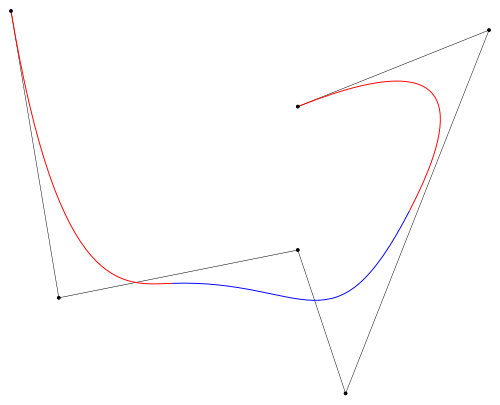
\includegraphics[width=0.50\textwidth]{../Imgs/B-spline_curve.png}
    \legend{Fonte: \citeonline{b_spline}}
\end{figure}


\section{Análise de Algoritmos}

A análise de algoritmos é o processo de se identificar uma formula matemática que melhor represente o custo de
utilização de uma dado algoritmo, podendo ser o tempo que o algoritmo leva para terminar com uma quantidade $n$
de dados, ou de espaço, quanto da memoria do computador o algoritmo ira usar durante seu processo.

Neste processo identificamos a qual fámilia de problemas esse algoritmo pertence, que corresponde ao seu custo de
computação \cite{introductionAlgorthms} e assim podemos categoriza-lo com báse na notação assintótica.

\begin{table}[htb]
	\centering
	\caption{\label{Notação Assintótica}Notação Assintótica}
	\begin{tabular}{|c|c|c|}
	\hline
		Complexidade & Nome & Eficiente \\ \hline
		$O(1)$ & Constante & Sim \\ \hline
		$O(log n)$ & Logartimica & Sim \\ \hline
		$O(n)$ & Linear & Sim \\ \hline
		$O(n log n)$ & "Linearitimica" & Sim \\ \hline
		$O(n^2)$ & Quadrática & Sim \\ \hline
		$O(n^3)$ & Cúbica & Sim \\ \hline
		$O(2^n)$ & Exponencial & Não \\ \hline
		$O(n!)$ & Fatorial & Não \\ \hline
	\end{tabular}
	\legend{Fonte: \cite{big_o_notation}}
\end{table}

A formula matemática identificada como a representação do custo computacional é "arredondada" para uma das familias
apresentadas acima, reduzindo a formula a sua caractereistica mais presente, visto que aqui assumimos que $n$ sejá
um valor muito grande. Por exemplos uma função que tenha a forma de $n^2 + n + c$, onde $c$ é uma constante, 
pode ser reduzida a $n^2$, já que está parte tera maior peso durante a computação, a caracterizando 
como $O(n^2)$, onde $O$ é a notação "O grande", que representa a complexidade do algoritmo \cite{introductionAlgorthms}.

Com está análise, encontramos um algoritmo que melhor se encaixe em determinado problema, antes de se
desenvolver o mesmo em uma linguagem de programação especifica, ou de utilizarmos algoritmos já implementados de forma
cega, podendo perder em tempo e em consumo desnecessário de memoria.

\subsection{Análise de Complexidade}

Na análise de complexidade, estimamos o tempo de execução de um algoritmo dado uma entrada de tamanho $n$, análisando 
seus comandos, como exemplo podemos utilizar o algoritmo de ordenação insertion sort. 

O insertion sort é um algoritmo eficiente para ordena uma sequência pequena de números, funciona de modo semelhante a
como muitas pessoas organizam cartas de um baralho na mão. Começamos com uma mão vazia, e a cada momento se pega uma
carta da mesa e se insere na mão em sua poisção correta, verificando da direita para a esquerda \cite{introductionAlgorthms}.

Recebendo um vetor $A[1..n]$ contendo a sequencia de tamanho $n$ que será ordenada,  o algoritmo representado pelo
psceudo código \ref{Insertion-Sort} ordena a sequencia encontrada no vetor $A$, tendo no máximo um valor da sequencia 
armazenado fora do vetor a cada dado momento, ao final, o vetor $A$, irá conter a sequencia ordenada \cite{introductionAlgorthms}.

\lstset{style=psceudo}
\begin{lstlisting}[caption={\label{Insertion-Sort}Insertion-Sort}]
	Insertion-Sort(A)
	for j = 2 to n
		jey = A[j]
		i = j - 1
		while i > 0 and A[i] > key
			A[i + 1] = A[i]
			i = i - 1
		A[i + 1] = key	
\end{lstlisting}
\legend{Fonte: \citeonline{introductionAlgorthms}}

Para visualizar a sequencia de passos que o insertion sort executa para a ordenação de dado vetor, 
tomemos o vetor $A = [5, 2, 4, 6, 1, 3]$, a sequência pode ser vista na imagem \ref{Operação do Insertion Sort}.

\begin{figure}[htb]
	\centering
	\caption{\label{Operação do Insertion Sort}Operação do Insertion Sort}
	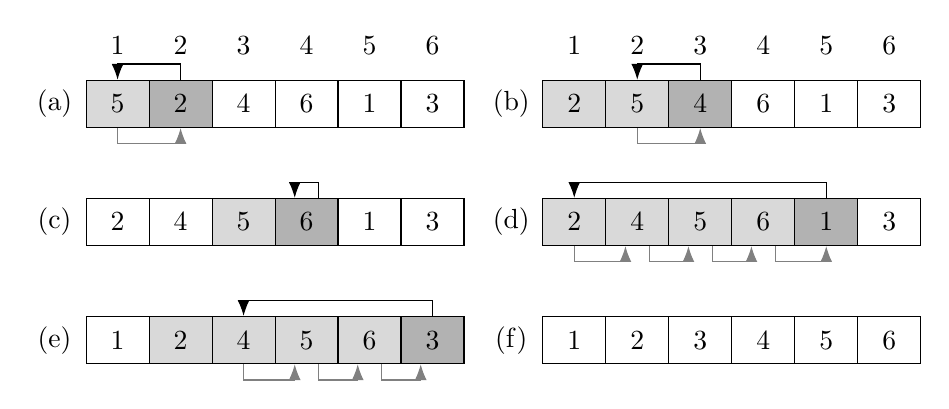
\begin{tikzpicture}[
		box/.style={draw, rectangle, minimum width=0.8cm, minimum height=0.6cm, align=center},
		label/.style={above=0.1cm},
		arrow/.style={draw, -{Latex[length=2mm,width=1.5mm]}}
	]

	% (a)
	\node at (0, 0) {(a)};
	\foreach \n/\c [count=\i] in {5/gray,2/black,4/white,6/white,1/white,3/white} {
		\node[box, fill=\c!30] (box-\i-a) at (\i * 0.8, 0) {\n};
		\node[label] at (\i * 0.8, 0.4) {\i};
	}
	\draw[arrow, color=gray] (box-1-a.south) -- ([yshift=-0.2cm]box-1-a.south) -| ([yshift=-0.2cm]box-2-a.south) -- (box-2-a.south);
	\draw[arrow, color=black] (box-2-a.north) -- ([yshift=0.2cm]box-2-a.north) -| ([yshift=0.2cm]box-1-a.north) -- (box-1-a.north);

	\vspace{0.5cm}

	% (b)
	\node at (5.8, 0) {(b)};
	\foreach \n/\c [count=\i] in {2/gray,5/gray,4/black,6/white,1/white,3/white} {
		\node[box, fill=\c!30] (box-\i-b) at (\i * 0.8 + 5.8, 0) {\n};
		\node[label] at (\i * 0.8 + 5.8, 0.4) {\i};
	}
	\draw[arrow, color=gray] (box-2-b.south) -- ([yshift=-0.2cm]box-2-b.south) -| ([yshift=-0.2cm]box-3-b.south) -- (box-3-b.south);
	\draw[arrow, color=black] (box-3-b.north) -- ([yshift=0.2cm]box-3-b.north) -| ([yshift=0.2cm]box-2-b.north) -- (box-2-b.north);

	\vspace{0.5cm}

	% (c)
	\node at (0, -1.5) {(c)};
	\foreach \n/\c [count=\i] in {2/white,4/white,5/gray,6/black,1/white,3/white} {
		\node[box, fill=\c!30] (box-\i-c) at (\i * 0.8, -1.5) {\n};
	}
	\draw[arrow, color=black] ([xshift=0.15cm]box-4-c.north) -- ([xshift=0.15cm, yshift=0.2cm]box-4-c.north) -| ([xshift=-0.15cm, yshift=0.2cm]box-4-c.north) -- ([xshift=-0.15cm]box-4-c.north);

	\vspace{0.5cm}

	% (d)
	\node at (5.8, -1.5) {(d)};
	\foreach \n/\c [count=\i] in {2/gray,4/gray,5/gray,6/gray,1/black,3/white} {
		\node[box, fill=\c!30] (box-\i-d) at (\i * 0.8 + 5.8, -1.5) {\n};
	}
	\draw[arrow, color=gray] (box-1-d.south) -- ([yshift=-0.2cm]box-1-d.south) -| ([xshift=-0.15cm, yshift=-0.2cm]box-2-d.south) -- ([xshift=-0.15cm]box-2-d.south);
	\draw[arrow, color=gray] ([xshift=0.15cm]box-2-d.south) -- ([xshift=0.15cm, yshift=-0.2cm]box-2-d.south) -| ([xshift=-0.15cm, yshift=-0.2cm]box-3-d.south) -- ([xshift=-0.15cm]box-3-d.south);
	\draw[arrow, color=gray] ([xshift=0.15cm]box-3-d.south) -- ([xshift=0.15cm, yshift=-0.2cm]box-3-d.south) -| ([xshift=-0.15cm, yshift=-0.2cm]box-4-d.south) -- ([xshift=-0.15cm]box-4-d.south);
	\draw[arrow, color=gray] ([xshift=0.15cm]box-4-d.south) -- ([xshift=0.15cm, yshift=-0.2cm]box-4-d.south) -| ([yshift=-0.2cm]box-5-d.south) -- (box-5-d.south);
	\draw[arrow, color=black] (box-5-d.north) -- ([yshift=0.2cm]box-5-d.north) -| ([yshift=0.2cm]box-1-d.north) -- (box-1-d.north);

	\vspace{0.5cm}

	% (e)
	\node at (0, -3.0) {(e)};
	\foreach \n/\c [count=\i] in {1/white,2/gray,4/gray,5/gray,6/gray,3/black} {
		\node[box, fill=\c!30] (box-\i-e) at (\i * 0.8, -3.0) {\n};
	}
	\draw[arrow, color=gray] (box-3-e.south) --  ([yshift=-0.2cm]box-3-e.south) -| ([xshift=-0.15cm, yshift=-0.2cm]box-4-e.south) -- ([xshift=-0.15cm]box-4-e.south);
	\draw[arrow, color=gray]  ([xshift=0.15cm]box-4-e.south) -- ([xshift=0.15cm, yshift=-0.2cm]box-4-e.south) -| ([xshift=-0.15cm, yshift=-0.2cm]box-5-e.south) -- ([xshift=-0.15cm]box-5-e.south);
	\draw[arrow, color=gray]  ([xshift=0.15cm]box-5-e.south) -- ([xshift=0.15cm, yshift=-0.2cm]box-5-e.south) -| ([xshift=-0.15cm, yshift=-0.2cm]box-6-e.south) -- ([xshift=-0.15cm]box-6-e.south);
	\draw[arrow, color=black] (box-6-e.north) -- ([yshift=0.2cm]box-6-e.north) -| ([yshift=0.2cm]box-3-e.north) -- (box-3-e.north);

	\vspace{0.5cm}

	% (f)
	\node at (5.8, -3.0) {(f)};
	\foreach \n/\c [count=\i] in {1/white,2/white,3/white,4/white,5/white,6/white} {
		\node[box, fill=\c!30] (box-\i-f) at (\i * 0.8 + 5.8, -3.0) {\n};
	}

	\vspace{0.5cm}

	\end{tikzpicture}

	\legend{Fonte: \citeonline{introductionAlgorthms}}

\end{figure}

A figura \ref{Operação do Insertion Sort}, mostra que o algoritmo \ref{Insertion-Sort} funciona para se ordenar um vetor,
onde, no inicio de cada interação do loop for, controlado pelo valor de $j$, o subvetor de elementos $A[1..j-1]$ consiste
de uma sequência ordenada, e os valores restantes $A[j+1..n]$ são os elementos ainda não verificados e $j$ é o elemento
que está sendo verificado \cite{introductionAlgorthms}.

Agora com o algoritmo \ref{Insertion-Sort}, conseguimos analisar o custo computacional do insertion sort, mas primeiro
precisamos definir, dois conceitos, "tempo de execução" e "tamanho da entrada", que segundo \cite{introductionAlgorthms} é:

\begin{itemize}
	\item Tamanho da entrada: Varia dependo do problema a ser abordado, porém é comumente o numero de items na entrada,
	por exemplo, o tamanho do vetor $A$.
	\item Tempo de execução: É o número de operações ou 'paços' executados, aqui desconsideramos o hardware, e assumimos
	que mesmo cada paço leva um tempo diferente de outras, o tempo da do $i$ paço é sempre uma constante, $c_i$.  
\end{itemize}

Em nosso algoritmo \ref{Insertion-Sort}, para cada $j = 2, 3, ..., n$, dizemos que $t_j$ representa o número de vezes que
o loop \textbf{while} da linha 5 foi executado, para cada valor de $j$. Sempre que temos um loop for ou while o teste é
executado uma vez a mais doque o corpo do loop.

Assim conseguimos chegar aa seguinte analise do algoritmo \ref{Insertion-Sort}:

\begin{table}[h!]
	\centering
	\caption{\label{Análise-Insertion-Sort} Análise Insertion Sort}
	\begin{tabular}{lll}
		\textbf{Linha} & \textbf{Custo} & \textbf{Vezes} \\
		2 & $c_2$ & $n$ \\
		3 & $c_3$ & $n-1$ \\
		4 & $c_4$ & $n-1$ \\
		5 & $c_5$ & $\sum_{j=2}^{n} t_j$ \\
		6 & $c_6$ & $\sum_{j=2}^{n} (t_j - 1)$ \\
		7 & $c_7$ & $\sum_{j=2}^{n} (t_j - 1)$ \\
		8 & $c_8$ & $n-1$ \\
	\end{tabular}
	\legend{Fonte: \citeonline{introductionAlgorthms}}
\end{table}

O tempo de execução total do algoritmo será a soma dos tempos de cada linha, onde uma linha que leve $c_i$ paços para executar
e execute $n$ vezes ira contribuir com $c_in$ para o tempo total de execução. Para encontrar o tempo de execução do insertion-
sort \ref{Insertion-Sort}, em uma entrada de tamanho $n$, somamos o produto do Custo e Vezes da tabela \ref{Análise-Insertion-Sort}:

\begin{equation}
	\label{tempo-execução-insertion-sort}
	T(n) = c_2n + c_3(n - 1) + c_4(n - 1) + c_5\sum_{j=2}^{n} t_j + c_6\sum_{j=2}^{n} (t_j - 1) + c_7\sum_{j=2}^{n} (t_j - 1) + c_8(n-1)
\end{equation}

O tempo de execução de um algoritmo vária dependendo do dado de entrada, onde podemos cair nó melhor ou pior caso, durante a
analise de complexidade, se leva em consideração apenas o pior caso \cite{introductionAlgorthms}, onde, no nosso caso de exemplo, 
o algoritmo será executado por completo percorrendo cada elemento do vetor, que ocorre quando o vetor se econtra em ordem decrescente.

O pior caso no algoritmo \ref{Insertion-Sort}, pode ser representado pela seguinte equação:

\begin{equation}
	\label{pior-caso-insertion-sort}
	\begin{split}
		T(n)&= c_2n + c_3(n - 1) + c_4(n - 1) + c_5(\frac{n(n+1)}{2}-1) + \\ 
			&c_6(\frac{n(n-1)}{2}) + c_7(\frac{n(n+1)}{2}) + c_8(n-1) \\
			&= (\frac{c_5}{2} + \frac{c_6}{2} + \frac{c_7}{2})n^2 + (c_2 + c_3 + c_4 + \frac{c_5}{2} - \\
			&\frac{c_6}{2} - \frac{c_7}{2} + c_8)n - (c_3 + c_4 + c_5 + c_8) \\
	\end{split}
\end{equation}

Podemos expressar a equação \ref{pior-caso-insertion-sort}, como $an^2 + bn - c$, para constantes $a, b$ e $c$, que dependem do custo de
$c_i$, mas é a taxa de crescimento que realemente nos interesa, logo consideramos apenas o maior termo da equação, isto é $an^2$, já que
os outros termos são insignificantes para valores muitos grandes de $n$. Com isto, ficamos com o fator de $n^2$ para o crescimento, portanto
o pior caso de tempo de execução como $\theta(n^2)$.

Agora para encontramors a qual classe apresentada na tabela \ref{Notação Assintótica} o algoritmo \ref{Insertion-Sort} pertence, convertemos
da notação $\theta$ (theta) para a $O$ (O-grande), esta conversão é simples já que o grupo de problemas abordados pela notação $\theta$ engloba
a notação $O$, isto é $\theta(g(n)) \subseteq O(g(n))$ onde $g(n)$ é a função de crescimento ($n^2$), portanto, o algoritmo \ref{Insertion-Sort}
é $O(n^2)$ logo pertence ao grupo de probelmas Quadráticoss \cite{introductionAlgorthms}.

\subsection{Análise de Espaço}

Na análise de espaço, levamos em conta as váriaveis que o algoritmo utiliza e/ou cria, como por exemplo estruturas
auxiliares como vetores ou matrizes, conseguimos representar o consumo esperado de memória atravez de uma formula
matemática \cite{introductionAnalysis}, assim como ná análise anterior, como exemplo tomemos o algortimo bubble-sort.

No algoritmo de bubble-sort, temos as seguintes váriaveis:

\begin{itemize}
	\item $vetor$ a sequencia de $n$ inteiros;
	\item $i$ um valor inteiro que representa uma posição na sequencia;
	\item $j$ um valor inteiro que representa uma posição na sequencia;
\end{itemize}

Assim, o algoritmo não cria nenhuma variavel a mais durante sua execução, acarretando em um custo de memoria costante durante
a sua execução. Sendo o tamanho de 2 inteiros mais o tamanho de um inteiro multiplicado pelo tamanho $n$ da sequencia de
inteiros.

Logo o consumo de memoria pode ser descrito por uma função linear, $f(n) = n + 2$, onde $n$ é o tamanho da sequencia de
entrada.

\section{Linguagem R}

R foi desenvolvido e pensado como uma linguagem e ambiente para computação estatística e gráficos, possue a capacidade
de trabalhar com vários processos estatísticos, como modelagem linear e não-linear, testes classicos de estatística,
sériese temporais, entre outros, e ser altamente extensível \cite{ling_r}.

Devido ao seu desenvolvimento focado em aplicações de computação estatística, ser semelhante e compativel 
com a lingaugem S já existente, e capaz de atuar com códigos feitos nas linguagens C, C++ e Fortran \cite{ling_r},
tornou o R uma linguagem popular dentro da área de compuatação estatística \cite{linguagem_r}.

O ambiente do R, pode ser fácilmente incrementado, se utilizando de bibliotecas, nomeadas como packages, por padrão,
temos oito packages que são encontrados junto da distribuição comum do R, outros packages podem ser encontrados em sites
especializados na distribuição dos mesmos \cite{ling_r}.

Além de ser de facil incrementação, o ambeinte R, possue um interface de desenvolvimento gratuita, o R Studio, onde
a utilização da linguagem fica concnetrada em uma unica aplicação, facilitando a visualização dos dados, gráficos, alteração
e manutenção do código e packages \cite{rstudio}.

\subsection{Packages}

Packages, também conhecidos como bibliotecas ou pacotes, dentro do cenario de computação, se refere a agrupamentos de códigos
desenvolvidos por terceiros ou por si mesmo, para encapsular alguma atividade ou processo, que pode ser utilizado em mais
de um projeto.

Como exemplo, podemos utilizar os packages, mda e mgcv, presentes neste trabalho, o package mda engloba funções para se aplicar
um grupo de modelagem de dados, sendo estes o Mixture and Flexible Discriminant Analysis, Multivariate Adaptive Regression 
Splines (MARS) e Vector-response Smoothing Splines \cite{mda}, já o mgcv, engloba Generalized Additive Models e algumas de suas variações
, Generalized Cross Validation e similares \cite{mgcv}.

Estes packages permitem ao usuário, apenas chamar a função que representa o processo a ser executado, não precisando se preocupar com
os pormenores da execução em si, apenas passar os parametros necessários de modo correto.

\section{Trabalhos relacionados}



% ========================================================================
% DESENVOLVIMENTO
% ========================================================================
 \chapter{Desenvolvimento}

 Lorem ipsum dolor sit amet, consectetur adipiscing elit. Sed sollicitudin tempor sapien in maximus. Quisque in vulputate dui, ac vestibulum sem. Suspendisse urna velit, dapibus nec egestas a, rhoncus vitae neque. Mauris quis efficitur augue. Aliquam quis tellus eget orci aliquet aliquam. Sed luctus, quam vitae elementum malesuada, quam lacus imperdiet urna, sed ullamcorper libero magna non elit. Cras laoreet arcu a augue volutpat, suscipit pretium tellus tempus. Sed eros tortor, imperdiet eu neque id, interdum egestas tortor.

% ========================================================================
% RESULTADOS
% ========================================================================
 \chapter{Resultados}

 Lorem ipsum dolor sit amet, consectetur adipiscing elit. Sed sollicitudin tempor sapien in maximus. Quisque in vulputate dui, ac vestibulum sem. Suspendisse urna velit, dapibus nec egestas a, rhoncus vitae neque. Mauris quis efficitur augue. Aliquam quis tellus eget orci aliquet aliquam. Sed luctus, quam vitae elementum malesuada, quam lacus imperdiet urna, sed ullamcorper libero magna non elit. Cras laoreet arcu a augue volutpat, suscipit pretium tellus tempus. Sed eros tortor, imperdiet eu neque id, interdum egestas tortor.

% ========================================================================
% CONCLUSÃO
% ========================================================================
 \chapter{Conclusão}

 Lorem ipsum dolor sit amet, consectetur adipiscing elit. Sed sollicitudin tempor sapien in maximus. Quisque in vulputate dui, ac vestibulum sem. Suspendisse urna velit, dapibus nec egestas a, rhoncus vitae neque. Mauris quis efficitur augue. Aliquam quis tellus eget orci aliquet aliquam. Sed luctus, quam vitae elementum malesuada, quam lacus imperdiet urna, sed ullamcorper libero magna non elit. Cras laoreet arcu a augue volutpat, suscipit pretium tellus tempus. Sed eros tortor, imperdiet eu neque id, interdum egestas tortor.

 \section{Trabalhos Futuros}

\begin{itemize}
    \item Trabalho Futuro 1
    \item Trabalho Futuro 2
    \item Trabalho Futuro 3
\end{itemize}

\postextual

% ========================================================================
% BIBLIOGRAFIA
% ========================================================================
\bibliography{bibliografia.bib}

% ========================================================================
% APENDICES
% ========================================================================
\begin{apendicesenv}

\partapendices

\chapter{\label{AnexoA}Exemplo de seção de anexo}

\begin{lstlisting}
EXEMPLO DE CODIGO A SER ADICIONADO
\end{lstlisting}

\end{apendicesenv}

\end{document}